\subsection{Generalizations}

This section focuses on more general cases. In particular,

\begin{enumerate}
\item \textbf{Multiple Constraint}, i.e., in the case of

\begin{equation}
J=\int f(x,y_1,y_2,...,y_n,\dot y_1, \dot y_2,...,\dot y_n, \ddot y_1,...)
\end{equation}


\item \textbf{Variable Endpoints}
In previous cases, we used the key assumption that:
\end{enumerate}

\begin{framed}
\textbf{Fixed Endpoint Assumption}\\
The perturbation $\delta y$ is 0 at endpoints, hence all boundary/surface terms arising from integartion by parts may be ignored.
\end{framed}

We now relax this assumption but rather work out boundary conditions based on the stationary condition with variable endpoints. This assumption can in turn be applied to the resulting differential equations.

\begin{enumerate}[resume]
\item \textbf{Constrained Optimization} Often, the minimization of the action is subjected to physcial constraint. For instance, in the famous \textit{catenary problem}, we need to fix the length of the hanging chain.
\end{enumerate}

\subsubsection{Multiple Constraint}

\subsubsection{Variable Endpoints}

\subsubsection{Constraint Optimization}

\subsubsection{Exercises}

\paragraph{Elastic Rods}

\begin{framed}
\textbf{Elastic Rods}\\
\begin{itemize}
\item The \textbf{elastic energy per unit length} of a bent steel rod is given by

\begin{equation}
\frac{1}{2}\frac{YI}{R^2}
\end{equation}


Here Y is the \textit{Young's modulus} of the steel and $I$ is the moment of inertia of the rod's cross section about an axis through its centroid and perpendicular to the plane in which the rod is bent.
\end{itemize}

\begin{figure}[!htbp]
\centering
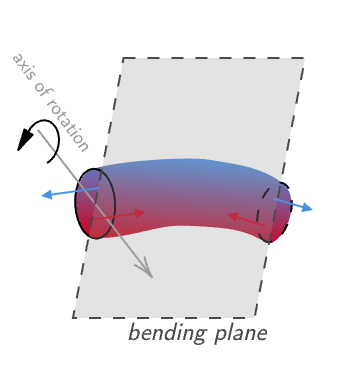
\includegraphics[width=0.375\linewidth]{files/bending_beam-3f593e81e849dc20a7466f2be18f704f.png}
\caption*{Bending beam and the axis of rotation associated with the moment of  inertia $I$}
\end{figure}

\begin{itemize}
\item Let us assume the rod is only slightly bent into the yz plane and lies close to the z axis. R is the radius of curvature due to the bending, related to the curvature by

\begin{equation}
\frac{1}{R}=\kappa = |T_z|
\end{equation}


where $T$ is the unit tangent vector to the rod.
\end{itemize}

\subparagraph{Problem 0}

Show that the elastic energy can be approximated by:
\begin{equation}
\boxed{U[y]=\int_0^L \frac12 \left\{ \frac{1}{2} YI(y'')^2 \right\}dz}
\end{equation}

\subparagraph{Problem 1}

The rod is used as a column which supports a compressive load $Mg$ directed along the z axis (which is vertical). Show that :

\textbf{(a)} when the rod buckles slightly (i.e. bends with both ends remaining on the z axis) the
total energy, including the gravitational potential energy of the loading mass M, can be
approximated by
\begin{equation}
\boxed{U[y]=\int_0^L \left\{ \frac{YL}{2} (y'')^2 - \frac{Mg}{2}(y')^2\right\}dz}
\end{equation}

\textbf{(b)} By considering deformations of the form
\begin{equation}
y(z)=\sum_{n=1}^{\infty} a_n\sin(\frac{n\pi z}{L})
\end{equation}
show that the column is unstable to buckling and collapse once
\begin{equation}
Mg \geq \frac{\pi^2}{L^2}YI
\end{equation}

\subparagraph{}
\end{framed}

\begin{framed}
\textbf{Solution to Problem 0}\\
We need a little lemma(or recall from Calculus I):
\begin{equation}
\kappa = \frac{y''}{(1+y'^2)^{3/2}}
\end{equation}

For small perturbation $|y'|\ll 1$ hence $(1+y'^2)^{\frac32} \approx 1$ hence
$\kappa = \frac{1}{R}=(y'')$. Squaring it we have :
\begin{equation}
\frac{1}{R^2}=(y'')^2
\end{equation}
Hence:
\begin{equation}
dU=\frac12 YI (y'')^2 dz
\end{equation}
Integrating get us the desired result.

\begin{proof}[Proof of lemma]If we imagine we traverse along a curve $\Gamma$, the accelearation would be:
\begin{equation}
r''(z) &= \frac{d}{dz}\left(\frac{dr}{dz}\right) \\
&=  \frac{d}{dz}\left(\frac{ds}{dz}T\right)  \\
&= \frac{d^2s}{dz^2}T + \frac{ds}{dz}\frac{dT}{dz}
\end{equation}
Note that
\begin{equation}
\left\langle T, \frac{dT}{dz}\right\rangle=0
\end{equation}
since $|T|=1$. Therefore $r''(z)$ can be decomposed to a tangential component $\frac{d^2s}{dz^2}T$ and a centrepetal component $\frac{ds}{dz}\frac{dT}{dz}$.
Also, $\frac{dT}{dz}$ is co-linear with our quanitty of interest
\begin{equation}
\frac{dT}{dz}=\frac{dT}{ds}\frac{ds}{dz}
\end{equation}
Therefore:
\begin{equation}
\boxed{r''(z)= \frac{d^2s}{dz^2}T + \left(\frac{ds}{dz}\right)^2 \frac{dT}{ds}}
\end{equation}
We can isolate the centrepetal component by apply a cross product:
\begin{equation}
T\times r''(z) &= T \times \left(\frac{ds}{dz}\right)^2\frac{dT}{dz}
\end{equation}
Now :

\begin{enumerate}
\item (LHS) $T=(1,0,y')/ds$, hence $r''(z) = (0,0,y'')$. Hence the cross product is:

\begin{equation}
\frac{1}{\sqrt{1+y'^2}} (1,0,y')^T \times (0,0,y'')  = \frac{1}{\sqrt{1+y'^2}}(0,y'',0)^T
\end{equation}


\item (RHS) Since $T, \frac{dT}{dz}$ are orthogonal to each other and both lie in the x-z plane, we have:

\begin{equation}
T \times \left(\frac{ds}{dz}\right)^2\frac{dT}{dz} =  \left(\frac{ds}{dz}\right)^2 \textcolor{brown}{\left|\frac{dT}{dz}\right|} (0,1,0)^T
\end{equation}
\end{enumerate}

Now combining the above two equations, we get:
\begin{equation}
\frac{y''}{\sqrt{1+y'^2}}=\left(\frac{ds}{dz}\right)^2  \left|\frac{dT}{dz}\right|
\end{equation}
As desired.

\end{proof}
\end{framed}

\begin{framed}
\textbf{Solution to Problem 1}\\
\begin{figure}[!htbp]
\centering
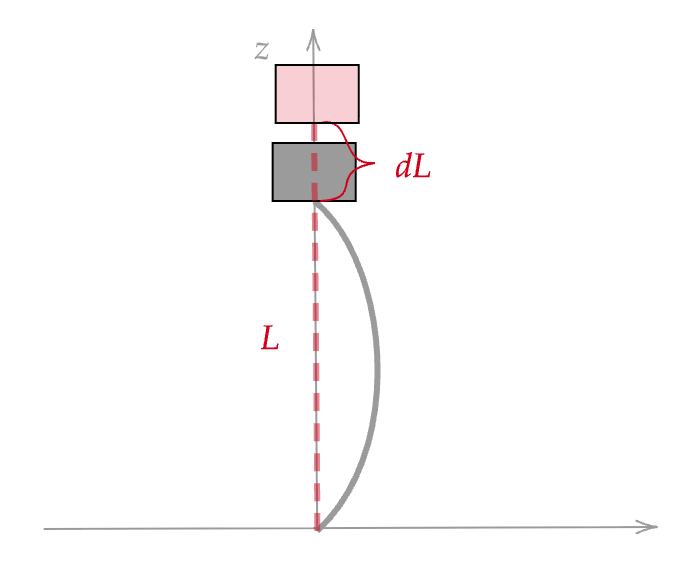
\includegraphics[width=0.7\linewidth]{files/euler_problem-85a6acb1fc4f4cee1ea1426b81e9491a.png}
\end{figure}

(a) Consider the schemetic above. Suppose $y=0$ for $z\in (L -dL,L)$, then
\begin{equation}
L+dL&=\int_0^L \sqrt{1+y'^2}dz \\ 
&\approx \int_0^L 1 + \frac{1}{2}y'^2dz\\
&= L + \int_0^L \frac{1}{2}y'^2dz
\end{equation}
Hence $dL=\int_0^L \frac{1}{2}y'^2$. If we consider the gravitational potential energy to be 0 at $h=L$, then the gravitational potential energy becomes:
\begin{equation}
-\int_0^L \frac{1}{2}y'^2dz
\end{equation}
the negative sign is there to account for compression. Combining with the result from problem 0 we get as desired.

(b) The Euler-Lagrange equation for the total energy functional is:
\begin{equation}
-\frac{d}{dx}\frac{\partial f}{\partial y'}+\frac{d^2}{dx^2}\frac{\partial f}{\partial y''} &= 0 \\
Mgy^{(2)}+YIy^{(4)} &= 0
\end{equation}

Consider a series solution of the form:
\begin{equation}
y(z)=\sum_{n=1}^{\infty} a_n\sin(\omega_n z)
\end{equation}
where $\omega_n = \frac{n\pi}{L}$. We have:

\begin{equation}
\widehat{\frac{\delta J}{\delta f}} &= \sum_{n=1}^{\infty}  b_n \sin(\omega_n z) \\
&= \sum_{n=1}^{\infty}\underbrace{a_n(YI\omega_n^4-Mg\omega_n^2)}_{b_n}\sin(\omega_n z)
\end{equation}

Hence a trivial solution is $a_n=0, \forall n\geq 1$ which corresponds to a \textit{stable, stiff rod}.

The rod buckles if, the trivial solution is no longer a local minimum, i.e., the hessian is no longer positive-definite. We need to find the hessian in this case.

Define the hessian in the spectral space as:

\begin{equation}
\widehat H = 
\begin{pmatrix}
\frac{\partial b_{1}}{\partial a_1} & \frac{\partial b_{1}}{\partial a_2} & \cdots \\
\frac{\partial b_{2}}{\partial a_1} & \frac{\partial b_{2}}{\partial a_2} & \cdots \\
\vdots  & & \ddots \\
\end{pmatrix}
\end{equation}

which in our case is already diagonalized:

\begin{equation}
\widehat H = \mathrm{diag}(\{(YI\omega_n^4-Mg\omega_n^2)\}_{n=1}^{\infty})
\end{equation}

Local minimum requires positive-definiteness, which is :
\begin{equation}
YI\omega_n^4 - Mg\omega_n^2 &> 0  \\
M &< \frac{YI}{g}\omega_n^2
\end{equation}

Picking $n=1$(smallest eigenvalue) satisfies the last inequality.
\begin{equation}
\boxed{M < \frac{YI\pi^2}{g L^2}}
\end{equation}

As desired.
\end{framed}